\documentclass[12pt]{article}
\usepackage[utf8]{inputenc}
\usepackage{biblatex}
\usepackage{graphicx}
\usepackage{amsmath}
\usepackage{amsfonts}
\usepackage{amssymb}
\addbibresource{references.bib}
\linespread{1.25}
\usepackage[lmargin=1.5in, rmargin=1.5in, tmargin=1in, bmargin=1in]{geometry}


\title{Thesis Interim Report}
\date{January 2017}
\author{Kevin Zhu}

\newlength\tindent
\setlength{\tindent}{\parindent}
\setlength{\parindent}{0pt}
\renewcommand{\indent}{\hspace*{\tindent}}
\setlength{\parskip}{1em}

\begin{document}
\begin{titlepage}
   \centering
   {\scshape\LARGE University of Toronto \par}
   \vspace{1cm}
   {\scshape\Large Thesis Interim Report\par}
   \vspace{1.5cm}
   {\huge\bfseries Geospatial Prediction for Goods Solicitation with Bayesian Data Fusion\par}
   \vspace{2cm}
   {\Large\itshape Kevin Zhu\par}
   \vfill
   supervised by\par
   Prof.~Scott \textsc{Sanner}
   \vfill
   {\large January 23, 2017\par}
\end{titlepage}

\newpage
\tableofcontents
\newpage

\section{Introduction}
% Context, gap and thesis purpose

% Introductory sentence
There is no single data set in the world that would allow one to get the statistical context for any kind of problem. One would usually have to retrieve information from different sources and piece them together to get a macroscopic idea of the problem space. This kind of data fusion will be explored in this thesis in the context of advertisements to solicit goods and donations. 

% Stuff about soliciting goods
Donations are a huge resource for non-government organizations for a variety of efforts. % Detail what kinds of organizations and what they do. 
Conventional strategies tend to gravitate towards a mass door-to-door solicitation of items or setups at a certain location and advertising to everyone to donate. %sentencing


% Background information
% What data is available. What are some other people doing. Understanding of the data
In order to solicit goods, one must understand who is willing to give away such items and at what time. Advertising to groups can be done on certain platforms like Facebook; however, they are severely limited in that they only provides tools to target certain demographics. Other platforms like Craigslist and Kijiji only provide information about item availabilities as well as location, but nothing about demographics. If one were to be limited to only one of these resources, gathering enough information to make availability predictions on a wide range of demographics would be impossible.

% Background on machine learning capabilities. 
% Bayes and Machine learning?
One particular method that can be used to make predictions is machine learning, as it is generally effective in the presence of an abundance of data. It can be used to learn the trends in categorical postings in Kijiji by cross referencing locations with census data in that location. On the other hand, without a sufficient or diverse training set, such models could potentially make wildly false predictions.

Another method that is conducive to querying is Bayesian Networks. <Stuff about Bayes Nets>

% Method
It is clear that data may only give information support part of the problem, therefore cross referencing and fusion with other data resources is necessary. Sources containing post information as well as locations can be fused with census data from the region of interest to generate probabilities of items becoming available in certain areas. Additional temporal information would support item predictions further into the future. While the data can be limiting, with Craigslist providing only posts and locations, and census data providing aggregate demographics of Toronto city wards, data fusion can be conducted to make inferences on an individual scale. This thesis paper will discuss a framework for Bayesian data fusion of posting data in Toronto with census data and compare it to more naive methods as well as some machine learning methods such as multi-class logistic regression. 



% Previous Material
   THIS IS PREVIOUS MATERIAL
   Local classifieds sites like Craigslist is a prime source for peer to peer selling of items. With 80 million classified ads being posted per month\cite{clfs}, the question of whether certain features that characterize the data set would allow for efficient learning of this group behaviour. While geospatial and temporal analysis has been conducted on data sets like crime [2] as well as disease [3], there has yet to be research utilizing both machine learning algorithms as well as geospatial predictive modeling. 

   The most modern methods of soliciting goods is through direct mail, door-to-door as well and online postings through Google Ads or Facebook Advertising. Physically mailing or going door-to-door have very clear drawbacks because the amount of time it requires to execute. While advertising platforms allows for wide targeting based on desired audience age, gender, estimated income level, marital and child status, the key question that emerges is how to target the demographics. This paper will describe and demonstrate an approach using Big Data to create user profiles for goods and services availability. 

   The problem with this approach is that credit card companies and retailers have purchaser info, but they do not make it accessible to other parties. It is very hard for third-party to gain cheap access to the data. Even if access were to be provided, the broad range of goods means that not one company or chain can give us the entire picture of habits. Finding the goods being bought is also very loosely related to the goods available for donation. Items that are purchased may not be donated anytime soon.

   A different approach is to observe a source that represents the availability of goods right from the beginning. Crawl community selling sites like Craigslist for latent goods availability. This solves previous concerns because it provides open and free access to data, broad coverage of goods and services and immediate availability of goods for donation. The problem that arises here is the hiding of personal details for privacy sake (and the fact that it's useless for the buyer). This presents the challenge to uncover features of the population that allow us to map between latent demographics of users and latent goods likely available for donation. 

   Successful predictions of items would have great benefits for day-to-day consumers who are looking for something relatively new at an affordable price, but the real implications lie within the organization and understanding of a monolithic data source.

   \subsection{Literature Review}
   % Review the state of the art, what has been accomplished and what hasn't been
   % Problems in current context and further detail
   % This is probably 2-3 pages
   % Lit Review topics
   % Solicitation of stuff. Importance of donaations, etc
   % Demographics predictions + verification
   % Feature Extraction/Cross referencing  
   % Population predictions
      
   \subsubsection{Introduction}
   % Transition between actual intro to this intro
   % State purpose
   % Establish organization
   While there hasn't been much study conducted on the methods best for the solicitation of goods, there's much research on methods to help with geospatial predictions in ecological studies. This review will investigate different motivations and strategies for geospatial analysis. 

   A conference presentation outlines the vast capabilities of machine learning and targets it towards geospatial prediction \cite{confpres}. Because of the vast number of variables present in geospatial problems, machine learning tends to find patterns and learn them very well. The presentation notes the possibility of training models using census data, allowing for fire risk to be predicted in Manhattan based on income, age and rent. The approach is heavily relevant to the thesis, as census data of Toronto can be used to predict goods availabilities throughout the city.

   One instance of landscape pattern analysis made use of neutral geographical models cross referenced with observed landscape patterns and ecological processes \cite{lpa}. Neutral models are defined as the minimum set of rules to generate patterns without the interference of another process \cite{neutralmodel}. This method is necessarily useful for gauging the effectiveness of a predictive model because of the comparison with a reference. A model's predictive capabilities may seem very impressive, but if the neutral model were to yield close to the same results, then it would be known that the added complexity of the constructed model would not have provided a worthwhile result. 

   Another paper studied the link between population dynamics with climate change. They observed population features such as population growth, migration, urbanization, aging and household composition \cite{popdyn}. The paper investigates different feature sets to aid the trend of climate change. The concept of feature extraction and investigation allows one to cross reference patterns characterized by a particular data set (climate change in this case) with a variety of feature sets. 

   The final instance makes use of Markov Random Fields as well as Spatial Autoregression models \cite{autoreg}. The paper takes a different approach from the first presentation's strictly feature learning model, as it takes a time series into account. The paper compares the standard Markov Random Field model for tying in spatial information to classification problems and the Spatial Autoregression model. 

   \subsubsection{Conclusion}
   Each paper was crucial to the overall understanding of the manipulation of geospatial elements with data for predictive purposes. Machine learning algorithms are simple to implement on problems with geospatial context due to the abundance of features that are present. While the concept of feature extraction was prevalent in the papers, they did not seem to consider techniques like heatmapping to visualize the data. These solutions have yet to be collectively employed as a holistic predictive system that can analyze features of an area and make predictions. While machine learning algorithms can certainly provide insight to patterns in a geographical area, SAR models can possibly be more accurate since it takes time series into consideration. The comparison between simple machine learning models, SAR and the baseline model without any features would be interesting to investigate. 

   % EXPERIMENTS


   \section{Experiment methodology}
   With the goal to ultimately try to predict which locations of Toronto are productive in which products, the first step in the process is to create a model. In order to create a model, data must be gathered and processed such that a machine learning model like multiclass logisitic regression can learn from the training data. 

   \subsection{Data Source}
   The data collection would be done on a single website to eliminate the variables in inconsistency and productivity between different websites. One could gather data from Ebay and Amazon; however, the postings are mostly from larger vendors, which does not suit the needs of thesis. Craigslist and Kijiji, on the other hand, are suitable because they are well known as "local classifieds", allowing anyone to post item listings for free. Since Craigslist is more widely known, it has been chosen for data collection. 

   \subsection{Data Description}
   The data collected should have geotags associated so that it is possible to learn geospatial patterns. The geotags should be granular enough such that postings do not get geospatially bunched together. We need to describe places in Toronto beyond the most well known areas, so if the geotags are not specific enough, it would be nigh impossible to learn geospatial patterns. Ideally, the data would also have a tag associated with it so that it can be bundled with other similar postings. Categories, for example, serves as a good bucketing system for Craigslist postings. A very detailed timestamp is also required so that temporal analysis can be done is a possibility for future work and investigation.

   \subsection{Data Learning Method}
   In order to learn the scraped data, a multiclass logistic regression model is used. 

   \subsubsection{Logistic Regression}
   Logistic regression uses the sigmoid function coupled with a linear function of multiple independent variables to ultimately determine a binary outcome. The sigmoid function is as follows: 
   \[\frac{1}{1+e^{-z}}\]
   The z is a linear function of the form
   \[z = \beta_0 + \beta_1*x_1 + \beta_2*x_2 + \beta_3*x_3  + ...\]
   The \(x\) values represent independent variables. The \(\beta\) values represent the weights associated with each \(x\) value. The sigmoid function can be used to calculate the probability of the outcome being 0 or 1. Given a vector of independent variables as well as the associated weights, the sigmoid function produces a value between 0 and 1 representing the probability. A threshold, usually 0.5, can be applied such that beyond the threshold, the probability maps to an output of 1 and the reverse maps to an output of 0. 

   \subsubsection{Multiclass Logistic Regression}
   Multiclass Logistic Regression is an extension of Logistic regression where the output can be more than just be 0 and 1. The output becomes a vector of probabilities for each possible output class. A function known as softmax, or the normalized exponential function, is used to get the probabilities of each class. The maximum probability would indicate the most likely class, and therefore that class would be the output of MCLR. The softmax function looks like the following: 
   \[Pr(Y_i = K) = \frac{e^{\beta_K} \cdot X_i}{\sum_{k=1}^{K} e^{\beta_K} \cdot X_i}\]

   \subsection{Model Construction}
   The MCLR model would be constructed by learning a training set of 70\% of the gathered data. Each posts' category would be the output variable for the model. The independent variables, or parameters, of the function would represent features of different feature sets pulled from Toronto census data. With Toronto split into 44 wards, a feature set can be constructed for each  The census data provides counts for different age groups, gender, household type and family size. These numbers can be normalized with respect to each ward to create ward profiles. The age and gender feature sets would be split into buckets, whereas household type and family size would be split into type and size buckets respectively. These would represent the parameters for the MCLR model. Once the model is trained, it will attempt to predict the post categories given a vector of parameters representing the ward profile. 

   \subsubsection{Criteria for model accuracy}
   There are three methods of gauging the model accuracy in this report: raw prediction accuracy, hit rate of 5 and log likelihood. Raw prediction accuracy is measured as 
   \[\text{Accuracy} = \frac{\text{correct predictions}}{\text{total predictions}}\]

   Since MCLR calculates the softmaxes for each possible class, one could count the appearance of the correct output among the top 5 of the most likely classes as a "hit". The hit rate of 5 can be calculated as follows:
   \[\text{Hit Rate of 5} = \frac{\text{times category appeared in top five}}{\text{total predictions}}\]

   Another method of gauging model effectiveness is through negative log likelihood. This method essentially takes the negative log of the likelihood that the MCLR model gives for the correct category, and then sums it over the entire test set. With the goal of maximizing the likelihood for correct predictions, we would expect a good model to minimize the negative log likelihood and have a total of as close to 0 as possible. This method is also useful in better comparing different feature sets. Some feature sets may have poor accuracy, but they may be very confident in the predictions which turn out to be true. This can be observed using the negative log likelihood.  

   \section{Progress to date}

   \subsection{Data Collection}
   Craigslist does not make its posting history public. Moreover, there is no available resource online that has collected a workable number of postings for use in this thesis. As a result, a data collection system had to be created.

   The most time-efficient and workable method was to use a CL wrapper written by Julio Malegria \cite{clwrapper}, which abstracts the interface and makes automated post querying easy. A script was written to extract all the posts on the home page along with their geotags. The homepage for the "all" section contains 2500 postings at any given time. New posts bump the last post off the front page, making it invisible to the scraper. Because of the fact that it is impossible to search the entire history of Craigslist, there is the possibility that many latent variables in posting patterns would have an impact on the data gathered. In order to safely ignore the possibility that these factors exist, data was scraped from Craigslist every day at 3:00 am. 

   The data collected has a number of useful attributes associated with it: the description of the item in the form of a title, geotags indicating the location at which the item is being sold, the url to the posting which contains its designated category as well as a a timestamp indicating when it was posted. The category, a three letter code, can be extracted from the URL and aids in the bucketing of posts without the need for description processing. The geotag is extremely useful, since this gives each posting an extra dimension of workable information: its geographical location. The timestamp allows for some temporal analysis. 

   \subsection{Initial findings: Category distribution over Ward}
   One of the first things done upon completing the data collection was a visual inspection of whether anything appeared remotely interesting. The first level of data processing was processing the scraped post data and associating each with one of the 44 wards in Toronto. Due to the highly irregular shaping of the Toronto Wards, association was done using nearest neighbours. Each posting's geotag allows for the search of the closest ward centroid. While this may not be entire accurate, it is a very cheap and efficient way of bucketing the posts. Over 55,000 posts were processed and bucketed.

   \begin{figure}[h]
   \centering
   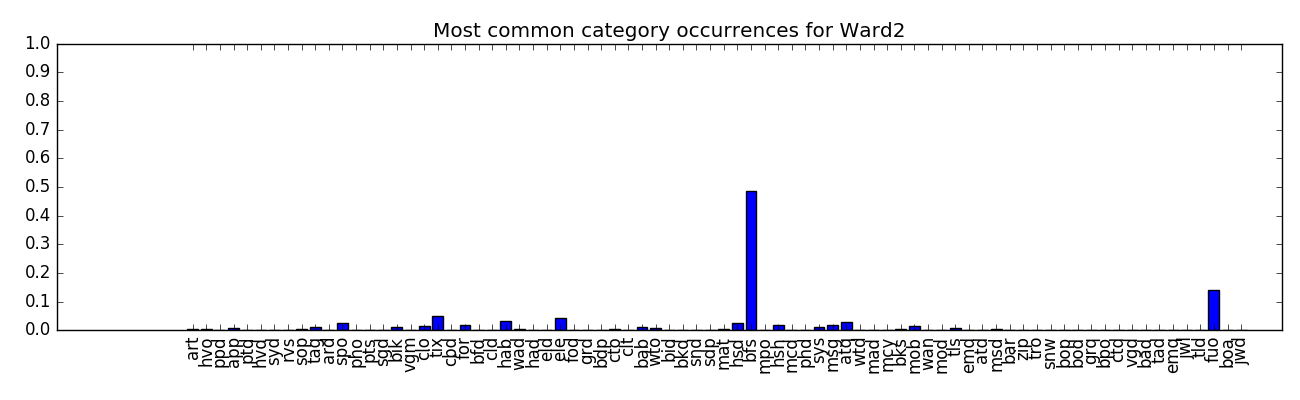
\includegraphics[width=14cm]{Ward_2.png}
   \caption{Categories of postings in ward 2}
   \end{figure}

   \begin{figure}[h]
   \centering
   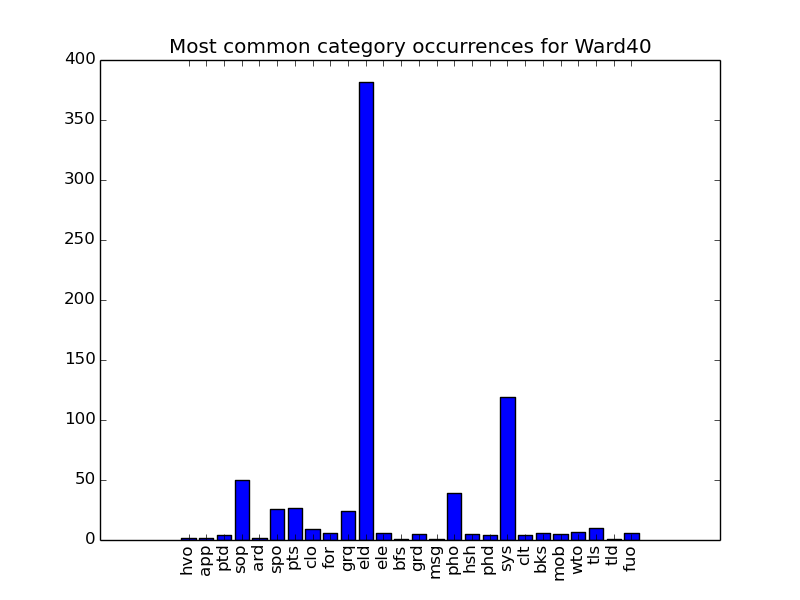
\includegraphics[width=14cm]{Ward_40.png}
   \caption{Categories of postings in ward 40}
   \end{figure}

   Graphing the distributions of categories of wards shows that in certain wards, very distinct peaks for different categories can be observed. This shows that there are features, latent or patent, that could help machine learning algorithms understand and predict posting locations. Had the resulting graphs shown largely random distributions of postings, it would not be immediately obvious that something could be learned. 

   \subsection{Learning Post Category through Toronto ward features}
   % This is basically P(Category|Demographic Distribution)
   Using census data from Toronto, it is possible to extract features for each ward. Age, female count, male count, family size and household type 
   Having bucketed the categories into wards. While it is difficult to spot particular idiosyncrasies with certain wards, these features can be fed into a multi-class logistic regression model. 

   The first feature set inspected was the age distribution of wards. There are 19 age groups containing a raw count of people falling in a particular group. For learning purposes, the age groups are normalized with respect to their ward totals. This removes discrepancies between wards caused by differing populations, and thus allows for a clear age profile. The logistic regression model takes in feature vectors, which are the age groups of a particular ward. The target would be the posting that emerged from that particular ward.

   % FORMULA Put in a latex formula x0 + wx1 + etc
   \[w_0 + w_1 \cdot x_1 + w_2 \cdot x_2 + w_3 \cdot x_3 + ...\]

   A notable caveat in this method is that, due to the fact that each ward can output posts form multiple different categories, the feature vector of age group would map to different categories. The natural consequence of this overlap is that the predicted outputs would be subject to inaccuracies. 

   % Establish the baseline.
   In order to ground the prediction accuracy of the model, a baseline must be established. Otherwise, it would be very difficult to establish just how effective a model is. 
   If one were to simply guess the category of a post, there would be a 1/78 chance of getting it right. If one were to guess the most common category of a ward, some wards would give under 20\% accuracy while some wards with heavy spikes, like ward 2 seen in figures 1 and 2 would have around 50\% accuracy. 

   % Put in the results of the learning here
   \begin{figure}[h]
   \centering
   \includegraphics[width=14cm]{results.png}
   \caption{Results of different feature sets.}
   \end{figure}
   The multiclass logistic regression is able to predict the post category with almost 20\% accuracy. This is reasonable, given the overlapping training set. 
   While accuracy is important for precise predictions, it would be of great use to view the top five categories of a ward to ensure that the model is indeed learning the features that define the ward and mapping it well to the categories that the ward outputs. The hit-rate of 5 is much higher than accuracy, showing that the post category is among the top 5 most probable categories for a ward almost 50\% of the time. 

   % Comparing different ward feature sets
   This experiment was run using each ward's female and male counts, household type as well as family size, all normalized by the ward total. 
   % Insert table about accuracy of different feature sets.
   It can be seen observed that household type and family size overall is less indicative of categories than age and gender. The log likelihood for each feature set is a great way of checking the confidence of the models formed by different feature sets. It could be that despite a lower accuracy with household type and family, their correct predictions may have higher probabilities. However, observing the negative log likelihood of the predictions by household type and family size features also reveals that they are poorer predictors with higher negative log likelihoods.

   % Heatmapping
   Another method of visualizing the raw collected data as well as the predictions is to heatmap the postings under a particular category.   
   The wards are not granular enough. As a result, it is nearly impossible to create telling heatmaps when the number of samples for a particular category is under a couple hundred. 

   \begin{figure}[h]
   \centering
   \includegraphics[width=6.3cm]{raw_clothing.png}
   \includegraphics[width=6cm]{predicted_clothing.png}
   \caption{Left: raw postings of the clothing category. Right: predicted "hotspots" for clothing postings.}
   \end{figure}

   The clothings posting had over 400 posts over the course of a month, allowing for predictions to show hot spots more prominently. While it does not completely reproduce the dense hot spots in the raw heatmap, it does manage to capture and display the densest regions for clothing postings. 

   % Talk about the weights of each age group
   Predicting accuracy and hit rate is useful in determining the correctness of a model. With confidence in the model, one could use it to investigate the particular features that best characterize the prevalence of a category.
   In multi-class logistic regression, the weights give a good indicator of how important a feature is to the overall model. Features that are very close to zero are not useful in terms of contribution to the probabilities of categories, whereas large features are very indicative of category decisions. 

   The following shows an example of features that play a large role in certain category determinations. 

   \begin{figure}[h]
   \centering
   \includegraphics[width=13cm]{stuff.png}
   \caption{The features that matter most for the determination of toys and games postings.}
   \end{figure}

   In Figure 5, the family of a single mother to a child is the most highly weighted feature. The second highest feature also has only 1 child. This could make potential sense since the child could easily outgrow his/her toys. With no child to pass it down to, it is likely to go up for sale. 
   While these results are interesting, and can make rudimentary sense, there is no method of verifying the correctness of the weights. The weights get noticeably smaller as one goes down the list, and so their meanings must be considered carefully. It is possible that features subsquent to the top contender are simply noisy outputs. 

   \newpage
   \section{Future Work: Experiments to perform //CHANGE THIS}

Due to the nature of the data collected from Craigslist, there is no way to obtain the granular details of the person making a particular post. Only post categories and the geotag would be given, making it impossible to verify predictions on the type of category posted by a particular demographic. 

In order to remedy this, we created a simulation of Toronto's activity on Craigslist. Using the 55000 data points scraped from Craigslist, normalized ward productivities can be created. This would allow for a "drawing samples from a bag" approach for the posts where the probability of a certain post being from a certain ward is the ward productivity over the 55000 data points. Using the ward population distributions for age extracted from census data, one could probabilistically generate the age group that the person making the post would fall in. 

Using this generative approach, 55000 new simulated data points were created on which Logistic Regression and Bayes Nets inferencing will be done.  


% PREVIOUS STUFF=====================================================================================================
   Currently, the training method was to randomly pick out 300 samples of data as the test set and use the remaning samples as a training set. While this is a reasonable method of training, it makes a big assumption on the data in that it stays consistent for the time in which the data is gathered. It is possible that population posting patterns drift overtime, and as such, a model trained on historical data may not be accurate in its predictions of future data. An experiment to conduct is to collect more data, and then use the 55,000 points in the past to predict categories posted by wards in the future. 

   % Simulations 
   The greatest challenge with the thesis does not lie within the construction of a model that can accurately predict posting categories, but rather the ability to verify the correctness of such a model. Currently, there is no efficient way of verifying whether such results are indeed representative of the population.

   From the data gathered over Craigslist, we can calculate the following:
   \[P(\text{category} | \text{demographics})\]
   % P(category | demographics)  

   In order to verify whether the predictions made are reputable, one could distribute surveys among the different wards in Toronto to construct the demographic profiles that are predicted by the multi-class logistic regression model. The however, would create great sample bias since individuals would largely choose to maintain their privacy. Furthermore, the possibility of false survey results remains an issue.

   In order to have full visibility of the demographic numbers, it is necessary to create a contained system modeling Toronto along with its wards and ward population behaviours. This way, one would be abel to observe the population distributions among a ward as well as each individuals. As a result, predictions about categories tied to age group can be confirmed by observing the actual preferences of age groups through synthetically created raw data. This would be the first course of action in the coming months. Afterwards, more time would be spent on creating an SAR model to incorporate time elements into the geospatial predictions. This model could be compared with the simple MCLR model in terms of accuracy. Further heatmaps will be created to make it easier to visualize the comparisons. 

   While the main project of simulating Toronto as well as creating a new model are underway, the MCLR model will continue to be tweaked with varying combinations of feature sets (combining male and female ward profiles for example). Furthermore, a new baseline model where no features are fed into it will be created to better quantify the role of different features in category predictions in a ward. 

   \section{Conclusion}

   Much of the analysis infrastructure for Toronto has been constructed up to this point. Preliminary model results are able to corroborate with prior stereotypical interpretations. Subsequent work will be done to improve the current MCLR model as well as explore additional models like SAR to process the data entirely differently. Because of the extreme difficulty of confirming the results of the models, it is necessary to create a simulated Toronto in order to cross check results with the actual population information, which is unavailable in reality. 
% END OF PREVIOUS STUFF=====================================================================================================


\newpage
\printbibliography

\end{document}
